\documentclass[times,10pt,twocolumn]{article} 
\usepackage{simpleConference}
\usepackage{times}

% Pour la commande onecolabstract (résumé 1 pleine largeur)
\usepackage{abstract}


%\usepackage[margin=2cm, columnsep=20pt]{geometry}
%\usepackage[affil-it]{authblk}
%\renewcommand{\abstractnamefont}{\normalfont\bfseries}
%\renewcommand{\abstracttextfont}{\normalfont\itshape}

% Pour les titres de section/sous-section
%\usepackage[compact]{titlesec}
%\titleformat{\section}{\large\bfseries}{\thesection}{1em}{}
%\titleformat{\subsection}{\normalsize\bfseries}{\thesubsection}{1em}{}
%\titleformat{\subsubsection}{\normalsize}{\thesubsubsection}{1em}{}


%\makeatletter
%\def\@maketitle{%
  %\newpage
  %\null
  %\vskip 2em%
  %\begin{center}%
  %\let \footnote \thanks
    %{\Large\bfseries \@title \par}%
    %\vskip 1.5em%
    %{\normalsize
      %\lineskip .5em%
      %\begin{tabular}[t]{c}%
        %\@author
      %\end{tabular}\par}%
    %\vskip 1em%
    %{\normalsize \@date}%
  %\end{center}%
  %\par
  %\vskip 1.5em}
%\makeatother

\usepackage[french]{babel}
\usepackage[T1]{fontenc}
\usepackage{lmodern}
\usepackage{csquotes}

\usepackage[backend=biber, style=nature, citestyle=authoryear]{biblatex}
\addbibresource{bibfile.bib}

\usepackage{amsmath}
\usepackage{amssymb}
\usepackage{mathtools}
\usepackage{amstext}
\usepackage{amsthm}
\usepackage{bbm}
\usepackage{fancyhdr}
\usepackage{siunitx}
\usepackage{physics}

\usepackage{xcolor}
\usepackage{hyperref}
\hypersetup{
    colorlinks,
    linkcolor={red!90!black},
    citecolor={blue!90!black},
    urlcolor={blue!90!black}
}


\usepackage{graphicx}
\usepackage{float}
\graphicspath{{figures/}} %Setting the graphicspath
\usepackage{float}
\usepackage{caption}
\usepackage{subcaption}
\usepackage{tabularx}
\usepackage{dcolumn}
\usepackage{booktabs}
\usepackage{makecell}


%\renewcommand\thesubsection{\alph{subsection})}
%\renewcommand\thesubsubsection{\Roman{subsubsection}}


\newcommand{\angstrom}{\textup{\AA}}
% Astronomy
\DeclareSIUnit\parsec{pc}
\DeclareSIUnit\lightyear{ly}

%Titre
\title{\vspace{-10mm}
\line(1,0){400}\\
Mesure de $H_0$ avec le quasar lentillé \textsc{RXJ1131-1231}
\line(1,0){400}
\vspace{-4mm}
}


%Auteur
\author{\large \textsc{Alexandre Adam}}
%\affil{Département de physique \\ Université de Montréal}
\affiliation{\vspace{2mm} PHY6669 -- Cosmologie\\
Département de physique \\ Université de Montréal
}
\date{\today}

\begin{document}
\twocolumn[
\maketitle
\begin{onecolabstract} % 10 points
\vspace{4mm} %
\end{onecolabstract}
]

\section{Introduction}\label{sec:intro}
\section{Lentilles Gravitationnelles}\label{sec:lens}
\subsection{Formalisme}
Dans cette section, on révise la théorie des lentilles gravitationnelles. 
Plus de détails peuvent être trouvés dans l'excellente revue de \cite{Treu2010}. \par

Une distribution de matière projeté sur le plan normal à la ligne de visée d'un 
observateur forme ce qu'on 
appel un champ de convergence $\kappa(\boldsymbol{\theta})$, où $\boldsymbol{\theta}$ sont 
les coordonnées angulaires du plan de la lentille. Ce champ génère un potentiel 
effectif $\psi(\boldsymbol{\theta})$ lié à $\kappa$ via une équation de Poisson
\begin{equation}\label{eq:Poisson} 
        \grad^{2}_{\boldsymbol{\theta}} \psi = 2 \kappa(\boldsymbol{\theta} ).
\end{equation} 
Cette équation est résolut en introduisant la fonction de Green appropriée

\begin{equation}\label{eq:Potentiel} 
        \psi(\boldsymbol{ \theta}) = \frac{1}{\pi} \int_{\mathbb{R}^2} 
        \kappa(\boldsymbol{ \theta}') \ln(\boldsymbol{\theta} - \boldsymbol{\theta}') d^2\boldsymbol{\theta}'.
\end{equation}
Il est pratique de rendre adimensionnel les quantités d'intérêts:
\begin{equation}\label{eq:Convergence} 
        \kappa(\boldsymbol{\theta}) \equiv \frac{\Sigma(\boldsymbol{\theta})}{\Sigma_{\mathrm{cr}}},
\end{equation} 
où on a introduit la densité de surface critique $\Sigma_{\mathrm{cr}}$
\begin{equation}\label{eq:Sigcritique} 
        \Sigma_{\mathrm{cr}} \equiv \frac{c^2}{4\pi G} \frac{D_s}{D_\ell D_{\ell s}}.
\end{equation}
On distingue 3 distances de diamètres angulaires $D_s$, $D_\ell$ et $D_{\ell s}$, 
soit la distance de l'observateur à la source, à la lentille et la distance 
entre la lentille et la source respectivement. Ces distances préservent les relations 
trigonométriques entre le plan source et le plan de la lentille, ce qui donne 
lieu à l'\textit{équation de la lentille}:
\begin{equation}\label{eq:LensEquation} 
        \boldsymbol{\beta} = \boldsymbol{\theta} - \boldsymbol{\alpha}(\boldsymbol{\theta}).
\end{equation} 
$\boldsymbol{\beta}$ représente les coordonnées angulaire dans le plan de la lentille et 
$\boldsymbol{\alpha}$ représente l'angle de deflection. Comme 
$\boldsymbol{\alpha}(\boldsymbol{\theta}) = \grad_{\boldsymbol{\theta}} \psi$, alors
\begin{equation}\label{eq:DeflectionAngle} 
        \boldsymbol{\alpha}(\boldsymbol{\theta}) = \frac{1}{\pi} \int_{\mathbb{R}^{2}} \kappa(\boldsymbol{\theta}')
        \frac{\boldsymbol{\theta} - \boldsymbol{\theta}^{'}}{|\boldsymbol{\theta} - \boldsymbol{\theta}'|}
        d^{2}\boldsymbol{\theta}'.
\end{equation} 
On note 
au passage que l'équation de la lentille est linéaire par rapport à $\boldsymbol{\beta}$, 
mais non-linéaire par rapport à $\boldsymbol{\theta}$. Cet aspect deviens important lorsqu'on 
cherche à optimiser la complexité numérique de la procédure d'optimisation des paramètres de la 
lentille. \par

L'équation de la lentille introduit deux effets de distortions, soit la magnification de l'image 
de la source et le cisaillement. Ces distortions sont décrites par la Jacobienne de 
l'équation de la lentille
\begin{equation}\label{eq:Jacobian} 
        A \equiv \frac{\partial \boldsymbol{\beta}}{\partial \boldsymbol{\theta}}
= \left( \mathbbm{1} - \frac{\partial^2 \psi}{\partial \theta_i \partial \theta_j} \right). 
\end{equation} 
Le cisaillement est un pseudo-vecteur $\gamma = (\gamma_1, \gamma_2)$ dans le plan de la lentille 
qui correspond à la partie antisymétrique et sans trace de la Jacobienne:
\begin{align}
        \gamma_1(\boldsymbol{\theta}) &=  \frac{1}{2} \left( \psi_{11} - \psi_{22} \right); \\
        \gamma_2(\boldsymbol{\theta}) &= \psi_{12} = \psi_{21}.
\end{align}
Ainsi, on peut modéliser les perturbations extérieurs au déflecteur principal de la lentille 
via l'effet de cisaillement en introduisant le potentiel extérieur qui correspond à un 
cisaillement constant:
\begin{equation}\label{eq:gamma_ext} 
        \psi_{\mathrm{ext}}  = \frac{1}{2} \gamma_{\mathrm{ext}} \theta^2 
        \cos 2(\varphi - \phi_{\mathrm{ext}}).
\end{equation} 
Le potentiel extérieur est exprimé en terme des coordonnées polaires du plan de la lentille 
$\boldsymbol{\theta} = (\theta, \varphi)$.

La magnification correspond à l'inverse du déterminant de la Jacobienne. 
\begin{equation}\label{eq:Magnification} 
        \mu \equiv \det{A}^{-1}.
\end{equation} 
Cette quantité peut être utilisé pour contraindre la luminosité de noyau actif de la galaxie 
source (AGN) via le ratio du flux des 4 images de l'AGN.
%Les valeurs 
%propres de la matrice de cisaillement sont $\pm \sqrt{\gamma_1^2 + \gamma_2^2 } = \pm \gamma$, 
%ainsi il est plus pratique d'introduire le cisaillement en coordonnée polaires $(\gamma, \phi)$:
%\begin{equation}\label{eq:JacobianDecomposition} 
        %A = (1 - \kappa)\mathbbm{1}
        %+ \gamma R(\phi).
%\end{equation} 


\subsection{Paramétrisation}
On paramétrise la densité surfacique de la lentille avec un profil elliptique avec une loi 
de puissance adouci:
\begin{equation}\label{eq:Kappa} 
        \kappa(\boldsymbol{\theta}) = \frac{3 - \gamma'}{2} 
        \left( 
        \frac{\theta_E}{\sqrt{q\theta_1^2 + \theta_2^2/q + \theta_c^2}}
\right)^{\gamma'- 1}. 
\end{equation} 
$\gamma'$ est la pente logarithmique radiale du profile, $q$ est le paramètre d'ellipticité
et $\theta_E$ est le rayon d'Einstein de la lentille. On introduit le rayon du coeur du profile 
$\theta_c$ pour éviter l'instabilité numérique du profile à l'origine du système de coordonnée. 
Il est pratique de fixer sa valeur à un angle plus petit que la taille angulaire d'un 
pixel de l'image (dans notre cas $\theta_c < 0.04''$). \par

Les intégrales \ref{eq:Potentiel} et \ref{eq:DeflectionAngle} ont une solution analytique 
seulement lorsque $\gamma'= 2$ (profil isotherme elliptique) ainsi que certains autres cas 
détaillés par \cite{Keeton2001}. En première approximation, ce paramètre peut être fixé 
à $2$ sachant que la plupart des systèmes de lentilles sont bien modélisé par ce profil. 
Laisser ce paramètre complètement libre requiert de procéder avec le traitement de 
\cite{Barkana1998}, où les intégrales dans le plan sont transformées en intégrales en une 
dimension. \par

On choisit une solution intermédiaire valide lorsque l'ellipticité de la lentille est 
petite (voir \cite{Barkana1998}). Le profil \texttt{SPEP} suppose que la forme 
du potentiel $\psi$ est identique à celle d'un profile isotrope (où 
les intégrales ont des solutions analytiques). Cette approche à l'avantage d'être plus 
rapide numériquement, au prix de développer des isocontours dans le potentiel $\psi$
en forme d'haltères lorsque 
l'ellipticité s'éloigne du domaine de validité.


%On choisit une solution intermédiaire informée du fait que la pente logarithmique 
%est très près d'une pente isotherme. Ainsi, on peut considérer une expansion de Taylor 
%au premier ordre autour de la solution isotherme. Cette approche à l'avantage d'être à 
%l'avantage d'être plus rapide à calculer numériquement. On doit toutefois restreindre 
%le domaine des valeurs possibles de $\gamma'$ à l'intervalle $\[1.6, 2.4\]$ où 
%l'erreur par rapport à la solution de Barkana 

\section{Délai temporels}
Le delai temporel est une mesure de la différence entre le temps d'arrivé d'une image $i$ 
et une image $j$ de l'AGN. Le formalisme des délai temporels introduit par une 
lentille gravitationnelle fut initialement introduit par \cite{Refsdal1964}. La même 
année, \cite{Shapiro1964} introduisait l'effet de dilation temporelle expérimenté par 
un photon traversant un champ gravitationnel. Les deux effets sont combinés dans ce 
qu'on appel le potentiel de Fermat:
\begin{equation}\label{eq:PotentielFermat} 
        \Psi_{\mathrm{Fermat}} = \frac{(\boldsymbol{\theta} - \boldsymbol{\beta})^{2}}{2}
        - \psi(\boldsymbol{\theta}).
\end{equation} 
Le délai entre deux images ($i$ et $j$) est donc mesuré par l'équation

%Un quasar est un objet idéal pour faire la mesure d'un délai 
%temporel en raison de la grande variabilité intrinsèque de sa luminosité 
%et sa petite 
%dimension physique ($\lesssim 10\mathrm{pc}$).



\begin{equation}\label{eq:TimeDelay} 
        c \Delta t_{ij} = D_{\Delta t} \left( \Psi_{\mathrm{Fermat, i}} - 
        \Psi_{\mathrm{Fermat, j}} \right),
\end{equation} 
où $D_{\Delta t}$ est la distance caractéristique du délai temporel
\begin{equation}\label{eq:Ddt} 
        D_{\Delta t} \equiv (1 + z_{\ell}) \frac{D_\ell D_s}{D_{\ell s}} \propto H_0^{-1}.
\end{equation} 
%\section{Méthodologie}\label{sec:metho}
%\subsection{}
\section{Observations de RXJ1131-1231}
La lentille gravitationnelle RXJ1131-1231 a été découverte par 
\cite{Sluse2003}. Des mesures spectroscopiques ont permis de déterminer le 
décalage vers le rouge de la source $z_s = 0.658$ et de la lentille 
$z_\ell = 0.295$ (\cite{Sluse2003}). Dans les prochaines sections, on détail 
la prise de mesure et le traitement \textit{a posteriori} des mesures pour 
extraire les données pertinentes à l'inférence.
\begin{figure}[H]
        \centering
        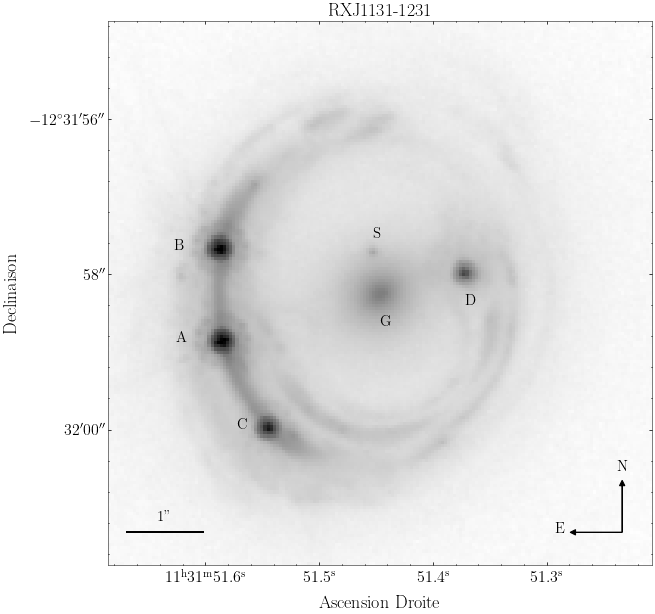
\includegraphics[width=\linewidth]{good_cutout}
        \caption{Image ACS \textit{drizzled} du système RXJ1131-1231 avec le filtre F814w obtenu 
                à partir de l'archive du télescope \textit{Hubble}. Les 
        4 images du quasar sont identifiés par les lettres A à D. Le déflecteur principal (G) 
        et son satellite (S) sont aussi identifiés. Les axes sont étiqueté par le système 
        de coordonnée céleste J2000.}
        \label{fig:rxj1131}
\end{figure}

\subsection{Traitement de l'image}
La prise de donnée consiste en 5 expositions de 1980.0 secondes avec 
l'instrument \texttt{ACS} du téléscope Hubble dans le filtre F814w. Ces 
expositions sont combinés par l'algorithme \texttt{MultiDrizzle} 
(voir \cite{Massey2010} et \cite{Koekemoer2007}) à une taille angulaire 
par pixel de $0.04''$.

Le bruit du compte d'électron dans chaque pixel
est modélisé à partir 
l'image de poids $w_{\mathrm{ACS}, i} = 1/\sigma^2_{\mathrm{ACS, i}}$ 
calculé lors du processus de 
\textit{drizzling} pour tenir compte de la corrélation du bruit de chaque pixel 
avec ses voisins lors du rééchantillionnage de l'image dans une grille de pixels 
effectifs.
Ces poids tiennent compte aussi
du fond noir du ciel, du courant noir du détecteur et des pixels saturés 
durant l'exposition (ainsi que des masques appliqués aux rayons cosmiques 
et traces laissées par des satellites).
\begin{figure}[H]
        \centering
        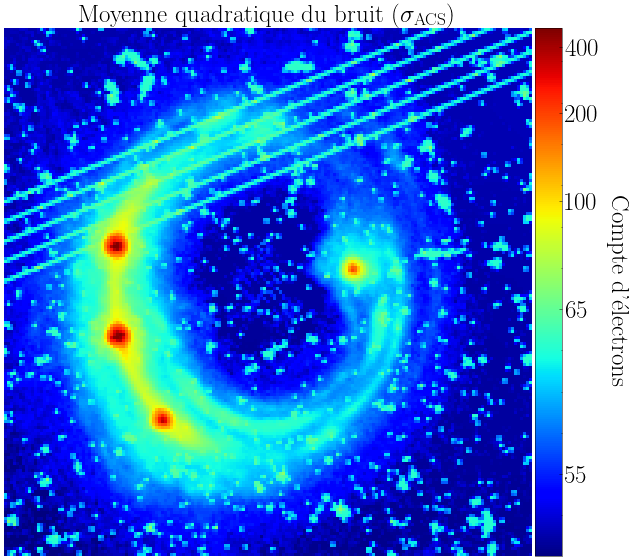
\includegraphics[width=\linewidth]{noise_map}
        \caption{}
        \label{fig:}
\end{figure}



\begin{figure}[H]
        \centering
        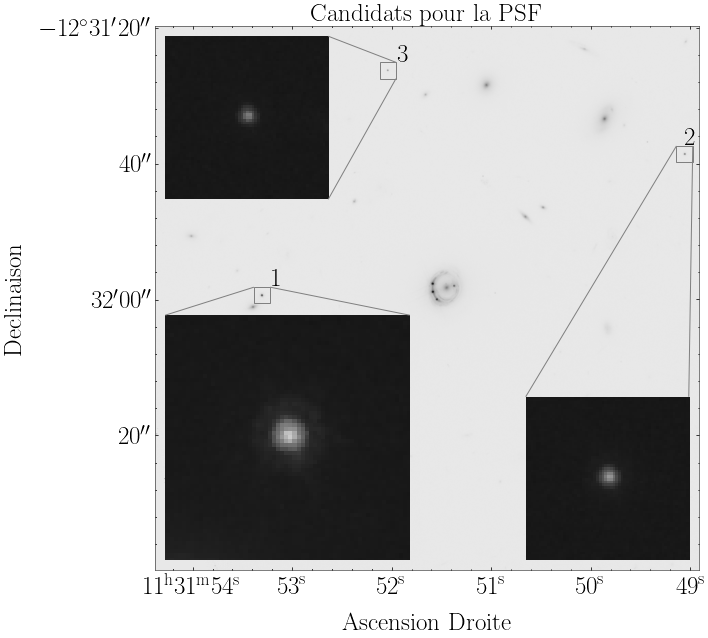
\includegraphics[width=\linewidth]{psf_cutout}
        \caption{}
        \label{fig:psf}
\end{figure}



\begin{align}
        \nonumber
        \log P(\underbrace{\mathbf{d}_{\mathrm{ACS}}}_{\mathcal{D}}
        | \underbrace{\theta_E, e, n, \boldsymbol{\gamma}, \mathbf{\eta}, \mathbf{s}}_{\mathcal{M}}) \propto  
        &-\frac{1}{2}\sum_{i=1}^{|\mathcal{D}|} \frac{(d_{\mathrm{ACS},i} - d_{\mathcal{M}, i})^{2}}
        {\sigma_{\mathrm{ACS},i}^2}
        \\
\label{eq:Inference} 
        &-\frac{1}{2}\sum_{i < j}^{4} \frac{(\boldsymbol{\beta}_{i} - \boldsymbol{\beta}_i)^{2}}{(d\theta)^{2}}
\end{align} 

\begin{align}
\nonumber
        \log P(\Delta t | D_{\Delta t}, \mathcal{M}) \propto 
        &-\frac{1}{2} \sum_i \frac{(\Delta t_i - \Delta t(D_{\Delta t, \mathcal{M}}))^{2}}{\sigma_{\Delta t}^{2}}
        \\\label{eq:JointLikelihood}
        &+\log P(\mathbf{d}_{ACS} | \mathcal{M})
\end{align}

\section{Résultats et discussion}\label{sec:resultats}
\begin{figure*}[hb]
        \centering
        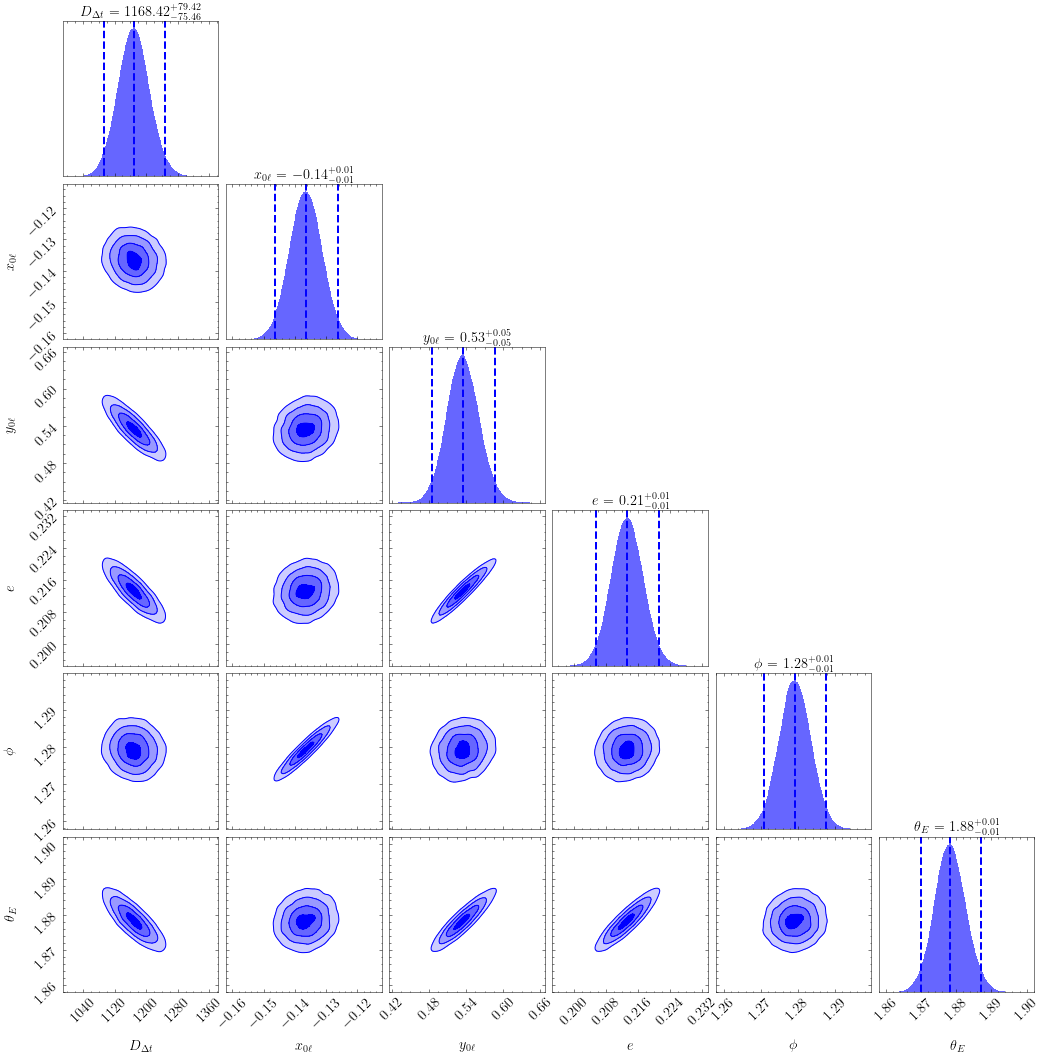
\includegraphics[width=0.8\textwidth]{corner_plot_joint}
        \caption{}
        \label{fig:cornerplot}
\end{figure*}

\begin{figure}[H]
        \centering
        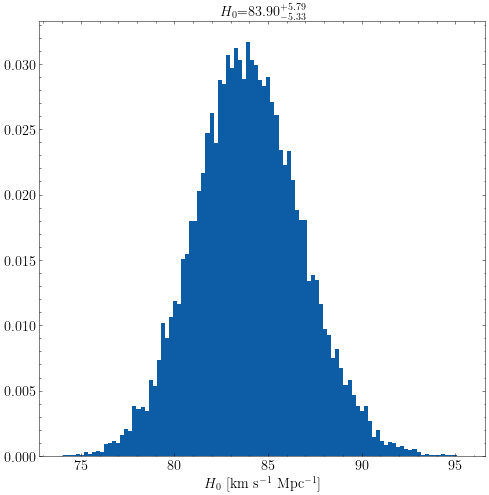
\includegraphics[width=0.8\linewidth]{marginalized_posterior_H0}
        \caption{}
        \label{fig:}
\end{figure}

\begin{table}[H]
        \centering
        \caption{Positions relatives des 4 images du quasar}
        \begin{tabular}{ccc}
                \toprule
                \thead{Images} & \thead{$\theta_1$\\ ($''$)} & \thead{$\theta_2$ \\ ($''$)} \\
                \midrule
                A & 1.8998 & 0.5659 \\\midrule
                B & 1.8717 & -0.6207 \\\midrule
                C & 1.2654 & -1.7385 \\\midrule
                D & -1.3217 & 0.2568 \\
                \bottomrule
        \end{tabular}
        \label{tab:}
\end{table}


\section{Conclusion}\label{sec:conclusion}

\printbibliography

\end{document}

